% Beamer-Klasse
\documentclass[aspectratio=43]{beamer} 	% 4:3 Format
%\documentclass[aspectratio=169]{beamer} % 16:9 Format

% Pakete laden
% Paket für Deutsche Sprache (Übersetzungen von Chapter zu Kapitel, 
% richtige Umlaute, richtige % Silbentrennung)
% siehe auch http://de.wikipedia.org/wiki/Babel-System
\usepackage[ngerman]{babel}

% Eingabecodierung, deutsche Umlaute oder die akzentuierten Zeichen sind verfügbar 
% und können direkt eingegeben werden
% siehe auch http://de.wikipedia.org/wiki/UTF8
\usepackage[utf8]{inputenc}

% Ausgabeschriftart von LaTeX festlegen
% siehe auch http://de.wikibooks.org/wiki/LaTeX-Schnellkurs:_Erste_Schritte
\usepackage[T1]{fontenc}

% Standardpfad für Grafiken
\graphicspath{{logos/}{bilder/}}

% Paket zum Erstellen von Plots mit TikZ
\usepackage{pgfplots}
% immer die neueste Version benutzen
\pgfplotsset{compat=newest}
% Verbindung von Linien durch eine schräge Kante
\pgfplotsset{every axis/.append style={line join=bevel}}
% Formatvorlage für Präsentationen
\mode<beamer>{
	\pgfplotsset{
		beamer/.style={
			width=0.8\textwidth,
			height=0.45\textwidth,
			legend style={font=\scriptsize},
			tick label style={font=\footnotesize},
			label style={font=\small},
			max space between ticks=28,
		}
	}
}
\mode<handout>{
	\pgfplotsset{
		beamer/.style={
			width=0.8\textwidth,
			height=0.45\textwidth,
			legend style={font=\scriptsize},
			tick label style={font=\footnotesize},
			label style={font=\small},
			max space between ticks=25,
		}
	}
}
\mode<article>{
	\pgfplotsset{
		beamer/.style={
			width=0.8\textwidth,
			height=0.45\textwidth,
			max space between ticks=35,
		}
	}
}
% neue Größenvorlage für zwei Plots nebeneinander anlegen
\pgfplotsset{
	scriptsize/.style={
		width=0.34\textwidth,
		height=0.1768\textwidth,
		legend style={font=\scriptsize},
		tick label style={font=\scriptsize},
		label style={font=\footnotesize},
		title style={font=\footnotesize},
		every axis title shift=0pt,
		max space between ticks=25,
		every mark/.append style={mark size=7},
		major tick length=0.1cm,
		minor tick length=0.066cm,
	}
}
\pgfplotsset{
	small/.style={
		width=6.5cm,
		height=,
		tick label style={font=\footnotesize},
		label style={font=\small},
		legend style={font=\footnotesize},
		max space between ticks=30,
	}
}
% Legendeneintrage standardmäßig links ausrichten
\pgfplotsset{legend cell align=left}
% Hauptgitternetz zeichnen
\pgfplotsset{xmajorgrids}
\pgfplotsset{ymajorgrids}
% Anzahl der kleinen Teilstriche zwischen zwei großen Teilstrichen
%\pgfplotsset{minor x tick num={3}}
%\pgfplotsset{minor y tick num={3}}
% feines Gitternetz zeichnen
%\pgfplotsset{xminorgrids}
%\pgfplotsset{yminorgrids}
% nur nach den Achsen skalieren
\pgfplotsset{scale only axis}
% Farben wie in MATLAB definieren
\definecolor{matlab1}{rgb}{0,0,1}
\definecolor{matlab2}{rgb}{0,0.5,0}
\definecolor{matlab3}{rgb}{1,0,0}
\definecolor{matlab4}{rgb}{0,0.75,0.75}
\definecolor{matlab5}{rgb}{0.75,0,0.75}
\definecolor{matlab6}{rgb}{0.75,0.75,0}
\definecolor{matlab7}{rgb}{0.25,0.25,0.25}
% Farbreihenfolge wie in MATLAB definieren
\pgfplotscreateplotcyclelist{matlab}{
	{matlab1,solid},
	{matlab2,dashed},
	{matlab3,dashdotted},
	{matlab4,dotted},
	{matlab5,densely dashed},
	{matlab6,densely dashdotted},
	{matlab7,densely dotted}% dies unterdrückt einen Fehler
}
% Farbreihenfolge wie in MATLAB benutzen
\pgfplotsset{cycle list name=matlab}
% Farbreihenfolge von pgfplots benutzen
%\pgfplotsset{cycle list name=color list}
% nur Graustufen benutzen
%\pgfplotsset{cycle list name=linestyles}
% Strichstärke auf 1pt festlegen
\pgfplotsset{every axis plot/.append style={line width=1pt}}
% für deutsche Dokumente ein Komma benutzen
\addto\extrasngerman{\pgfplotsset{/pgf/number format/.cd,set decimal separator={{{,}}}}}
% ein halbes Leerzeichen als Tausendertrennzeichen benutzen
%\pgfplotsset{/pgf/number format/.cd,1000 sep={\,}}
% kein Tausendertrennzeichen verwenden
\pgfplotsset{/pgf/number format/.cd,1000 sep={}}
% Zahlen kleiner als 0.1 auch im fixed-Format ausgeben
\pgfplotsset{/pgf/number format/.cd,std=-2}
% neue Positionen für Legenden anlegen
\pgfplotsset{/pgfplots/legend pos/north/.style={/pgfplots/legend style={at={(0.50,0.97)},anchor=north}}}
\pgfplotsset{/pgfplots/legend pos/south/.style={/pgfplots/legend style={at={(0.50,0.03)},anchor=south}}}
\pgfplotsset{/pgfplots/legend pos/east/.style={/pgfplots/legend style={at={(0.97,0.50)},anchor=east}}}
\pgfplotsset{/pgfplots/legend pos/west/.style={/pgfplots/legend style={at={(0.03,0.50)},anchor=west}}}
\pgfplotsset{/pgfplots/legend pos/outer north/.style={/pgfplots/legend style={at={(0.50,1.03)},anchor=south}}}

% Paket für SI-Einheiten
\usepackage[load-configurations=binary]{siunitx}
% Trennzeichen für Bereiche
\addto\extrasngerman{\sisetup{range-phrase={ bis~}}} 
\addto\extrasenglish{\sisetup{range-phrase={ to~}}}

% Paket, um das Floating in Article-Modus abzuschalten
\usepackage{float}

% Paket, um anderen Zeilenabstand einzustellen, besonders für Tabellen
\usepackage{setspace}

% Paket für ein intelligentes Leerzeichen
\usepackage{xspace}

% Abkürzung für z. B.
\newcommand{\zB}{z.\,B.\xspace}

% Paket für schönere Brüche im Textmodus
\usepackage{xfrac}
% Standardeinstellung mit einem schrägen Bruchstrich
\UseCollection{xfrac}{plainmath}

% schönere Tabellen
\usepackage{booktabs}



% Datenquelle der Logos: http://www.cd.ovgu.de/

%===Design der Universität ===
% Otto-von-Guericke-Universität
\usepackage{style/beamer_ovgu}		% deutsch
%\usepackage{style/beamer_ovgu-en}	% english


%===Fakultäten Design / faculty design===
% Fakultät für Maschinenbau
% faculty of mechanical engineering
%\usepackage{style/beamer_mb} 		% deutsch
%\usepackage{style/beamer_mb-en}	 	% english 

% Fakultät für Verfahrens- und Systemtechnik
% faculty of process and system engineering
%\usepackage{style/beamer_vst}		% deutsch
%\usepackage{style/beamer_vst-en}	% english

% Fakultät für Elektrotechnik und Informationstechnik
% faculty of electrical engineering and information technology
%\usepackage{style/beamer_eit}		% deutsch
%\usepackage{style/beamer_eit-en}	% english

% Fakultät für Informatik
% faculty of computer science
%\usepackage{style/beamer_inf}		% deutsch
%\usepackage{style/beamer_inf-en}	% english

% Fakultät für Mathematik
% faculty of mathematics
%\usepackage{style/beamer_ma}		% deutsch
%\usepackage{style/beamer_ma-en}		% english

% Fakultät für Naturwissenschaften
% faculty of natural science
%\usepackage{style/beamer_nat}		% deutsch
%\usepackage{style/beamer_nat-en}	% english

% Medizinische Fakultät
% faculty of medicine
%\usepackage{style/beamer_med}		% deutsch
%\usepackage{style/beamer_med-en}	% english

% Fakultät für Humanwissenschaften
% faculty of human science
%\usepackage{style/beamer_hw}		% deutsch
%\usepackage{style/beamer_hw-en}		% english

% Fakultät für Wirtschaftswissenschaften
% faculty of economics and management
%\usepackage{style/beamer_ww}		% deutsch
%\usepackage{style/beamer_ww-en}		% english


%===weitere Designs===
% Stil des Lehrstuhls für Elektromagnetische Verträglichkeit laden
%\usepackage{beamer_emv}

% begin der Präsentation / begin presentation
\title[Kurztitel]{A Machine Learning Framework for Gait Classification Using Inertial Sensors:\newline {\small Application to Elderly, Post-Stroke and Huntington's Disease Patients}}
\author{Robert Kowal}

\institute[Lehrstuhl XYZ]{
	\medskip
	Scientific Working \\
	Medical Systems Engineering 2018\\
	Faculty of Electrical Engineering and Information Technology\\
	Otto-von-Guericke-Universität, Magdeburg
}
\mode<presentation>{\keywords{Schlüsselwörter durch Komma getrennt}}
\date[01.01.2016]%{Datum der Präsentation, \zB 1. Januar 2016}

\begin{document}

\begin{frame}
	\maketitle
	% \maketitle funktioniert auch im Article-Modus
	% \titlepage funktioniert nur bei Präsentationen
\end{frame}


\section{Introduction}

% nur für die Miniframe-Navigation
\subsection*{}



\begin{frame}

\frametitle {Gait Assessment}

\begin {block}{Analysis of physical mobility}
\end{block}

\medskip

\begin{block}{Important because}
\begin{itemize}
\item [$\triangleright$]essential for everyday life
\item [$\triangleright$]risk of fall
\item [$\triangleright$]need of a mobility aid
\item [$\triangleright$]success of therapy
\end{itemize}
\end{block}
\medskip

\begin{block}
{$\Rightarrow$ Automatic classification is wanted and needed}
\end{block}

\end{frame}





\begin{frame}

\frametitle {Inertial Sensors (IMUs)}

\begin{block}
{Accelerometer + Gyroscope}
\end{block}
\begin{figure}[!t]
\centering
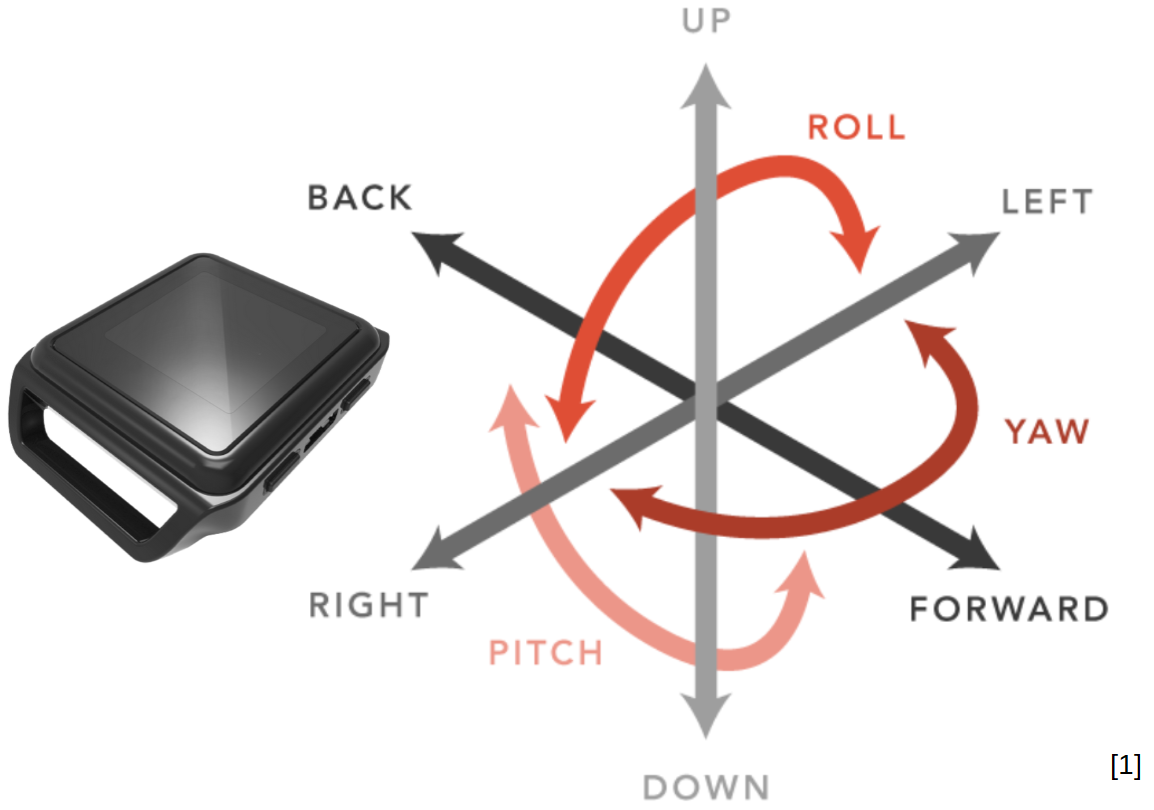
\includegraphics[height=3cm]{IMU.png}
\end{figure}
\begin{block}
{$\blacktriangleright$ minimal discomfort}
\end{block}

\begin{block}
{$\blacktriangleright$ useable in everyday life}
\end{block}

\end{frame}




\begin{frame}

\frametitle {Research so far {\rmfamily I}}

\begin{block} {Machine Learning applications}
\begin{itemize}
\item []
\item [$\triangleright$] classification of walking/jogging
\item []
\item [$\triangleright$] walking type (level/inclined/stair climb)
\item []
\item [$\triangleright$] gesture recognition
\item []
\item [$\triangleright$] user authentication
\end{itemize}
\end{block}

\end{frame}





\begin {frame}
\frametitle {Research so far {\rmfamily II}}

\begin{block}{Methods}
\begin{itemize}
\item []
\item [$\triangleright$] Hidden Markov Models (HMM)
\item []
\item [$\triangleright$] Support Vector Machines (SVM)
\item []
\item [$\triangleright$] Artificial Neural Networks (ANN)
\item []
\end{itemize}
\end{block}

\end {frame}




















\section{Research}

\subsection*{}
\begin{frame}
\frametitle {Goals of this research}

\begin{block}
{$\blacktriangleright$ machine learning framework for feature definition}
\end{block}

\begin{block}
{$\blacktriangleright$ combination of HMM and SVM}
\end{block}

\begin{block}
{$\blacktriangleright$ classification of pathological gaits\newline (post-stroke \& Huntington's)}
\end{block}


\begin{block}
{Future \newline $\Rightarrow$ embedded gait assessment for early detection}
\end{block}

\end{frame}







\begin{frame}
\frametitle {The Study}

\begin{columns}
\begin{column}{7.5cm}
\begin{block}
{42 Patients}
\end{block}

\begin{block}
{$\blacktriangleright$ 15 Post-Stroke (PS)}
\end{block}

\begin{block}
{$\blacktriangleright$ 17 Huntington's Disease (HD)}
\end{block}

\begin{block}
{$\blacktriangleright$ 10 Healthy Elderly (EL, control group)}
\end{block}
\end{column}
\begin {column}{2.4cm}
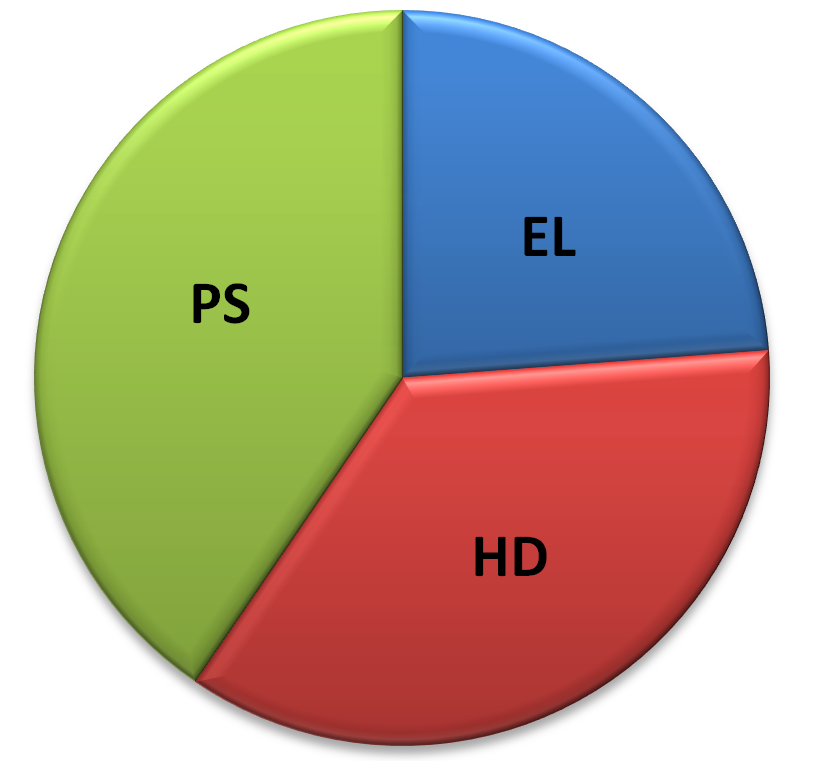
\includegraphics[height=2.8cm]{Study.png}
\begin{block}
{ }
\end{block}


\end{column}
\end{columns}

\end{frame}






\begin{frame}
\frametitle {Data generation}

\begin{columns}
\begin{column}{5.3cm}
\begin{block}
{ 3 IMUs }
\begin{itemize}
\item [$\triangleright$]left \& right shank
\item [$\triangleright$] waist
\item [$\Rightarrow$] 5Hz low-pass filtered
\end{itemize}
\end{block}
\begin{block}
{7m gait pressure mat}
\begin{itemize}
\item [$\triangleright$] foot strike
\item [$\triangleright$] toe off
\item [$\Rightarrow$] synchronization with IMUs
\end{itemize}
\end{block}

\end{column}

\begin{column}{5cm}
\begin{figure}[!t]
\centering
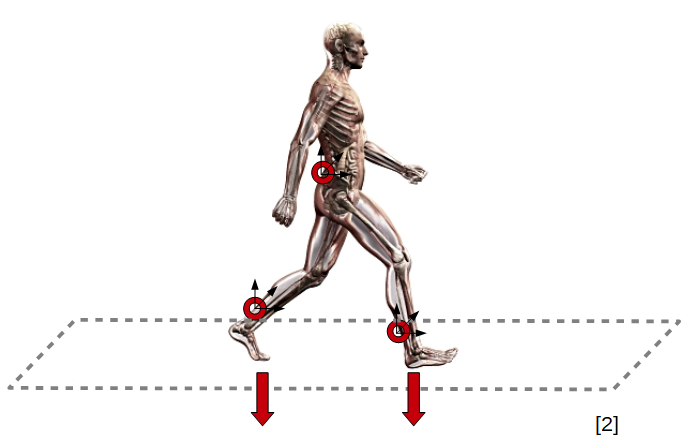
\includegraphics[height=3.4cm]{datageneration.png}
\end{figure}
\begin{block}
{}
\end{block}

\end{column}


\end{columns}
\end{frame}










\begin{frame}
\frametitle{Classification strategy}
\begin{figure}[!t]
\centering
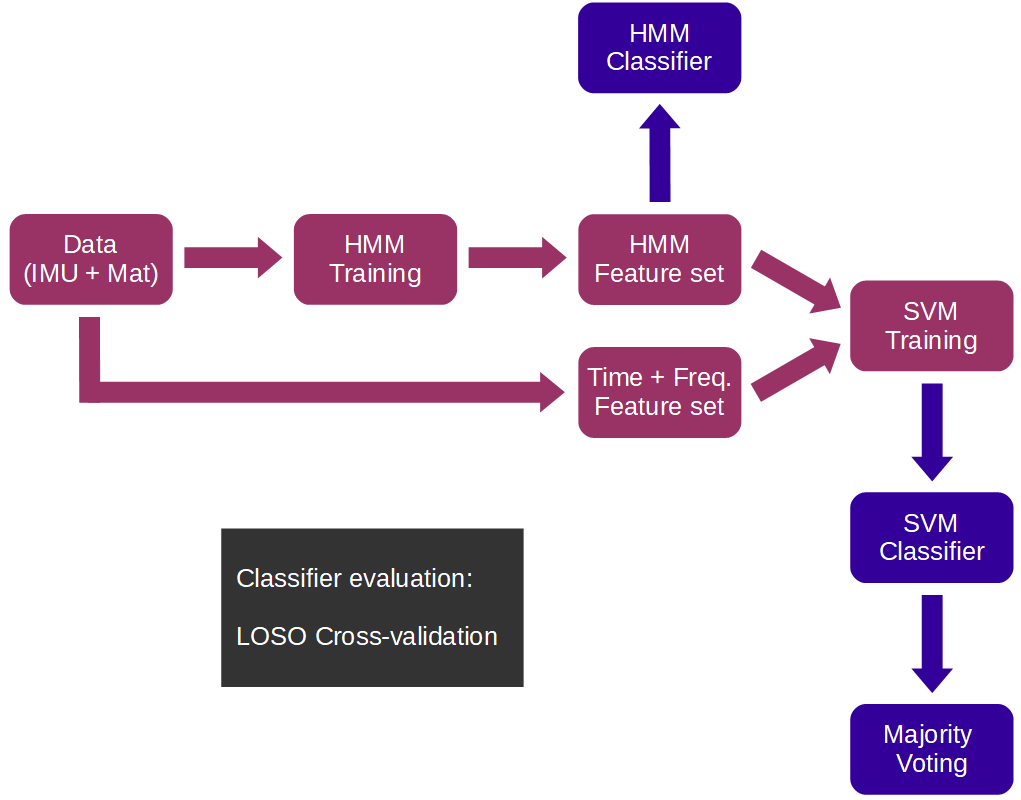
\includegraphics[height=6.6cm]{classificationstrategy.png}
\end{figure}
\end{frame}










\begin{frame}
\frametitle{Hidden Markov Models (HMM)}

\begin{columns}
\begin{column}{6.5cm}
\begin{block}
{$\blacktriangleright$ statistic based classifier}
\end{block}
\begin{block}
{$\blacktriangleright$ 1 HMM for each class trained}
\end{block}
\begin{block}
{$\blacktriangleright$ probability that sensor data fits one specific class}
\end{block}

\begin{block}
{\newline $\Rightarrow$ 66.7\% accuracy}
\end{block}

\end{column}

\begin{column}{3.6cm}
\begin{figure}[!t]
\centering
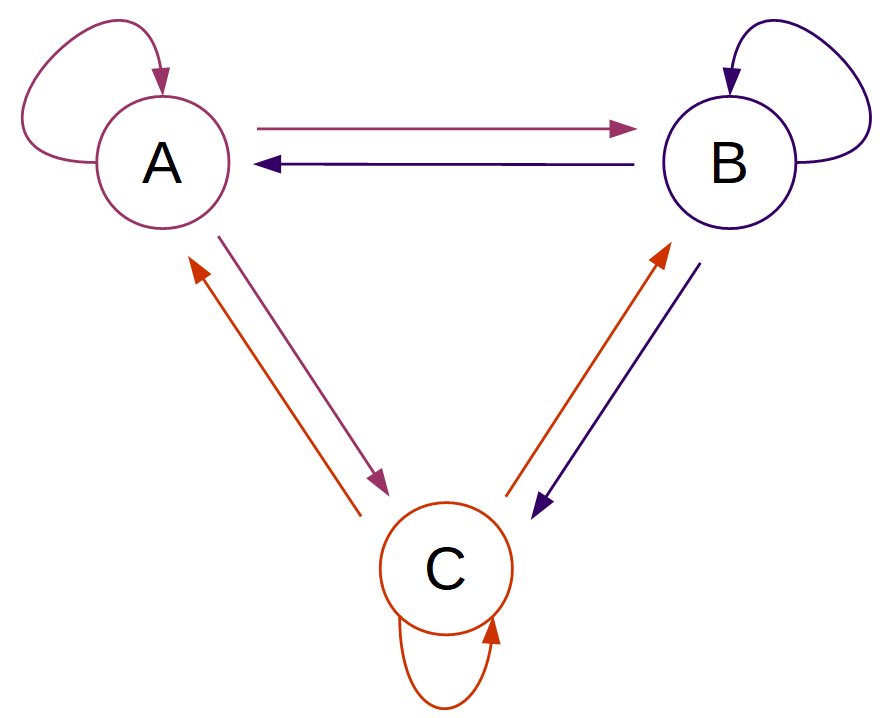
\includegraphics[height=3.3cm]{HMM.png}
\end{figure}
\begin{block}
{}
\end{block}
\end{column}
\end{columns}

\end{frame}









\begin{frame}
\frametitle{Support Vector Machine (SVM)}

\begin{columns}
\begin{column}{6.5cm}
\begin{block}
{$\blacktriangleright$ geometric classifier}
\end{block}
\begin{block}
{$\blacktriangleright$ division of feature space}
\end{block}
\begin{block}
{$\blacktriangleright$ decision based on position to hyperplane}
\end{block}



\end{column}

\begin{column}{3.6cm}
\begin{figure}[!t]
\centering
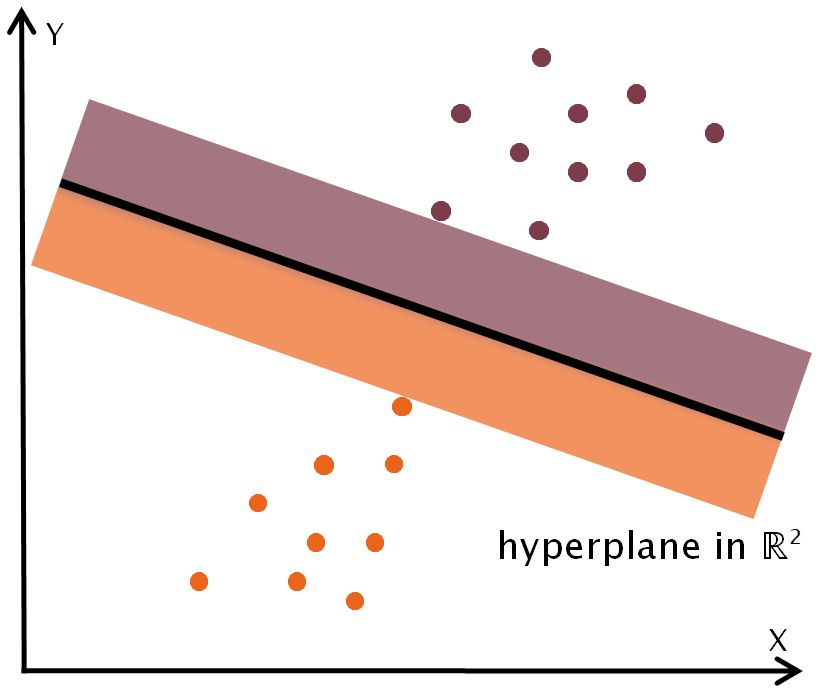
\includegraphics[height=3.3cm]{svm.png}
\end{figure}
\begin{block}
{}
\end{block}
\end{column}
\end{columns}

\end{frame}












\begin{frame}
\frametitle{SVM accuracies}

\begin{block}
{HMM-features only \newline $\Rightarrow$ 71.5\% accuracy}
\end{block}

\begin{block}
{time and frequency domain features only \newline$\Rightarrow$ 71.7\% accuracy}
\end{block}

\begin{block}
{both feature sets \newline$\Rightarrow$ 73.3\% accuracy}
\end{block}

\end{frame}









\begin{frame}
\frametitle{Majority Voting}

\begin{columns}
\begin{column}{6.5cm}
\begin{block}
{$\blacktriangleright$ aggregation of classifiers}
\end{block}
\begin{block}
{$\blacktriangleright$ 1 vote per classification}
\end{block}
\begin{block}
{$\blacktriangleright$ votes generated by passages}
\end{block}

\begin{block}
{\newline $\Rightarrow$ 90.5\% accuracy}
\end{block}
\begin{block}
{}
\end{block}

\end{column}

\begin{column}{3.6cm}
\begin{figure}[!t]
\centering
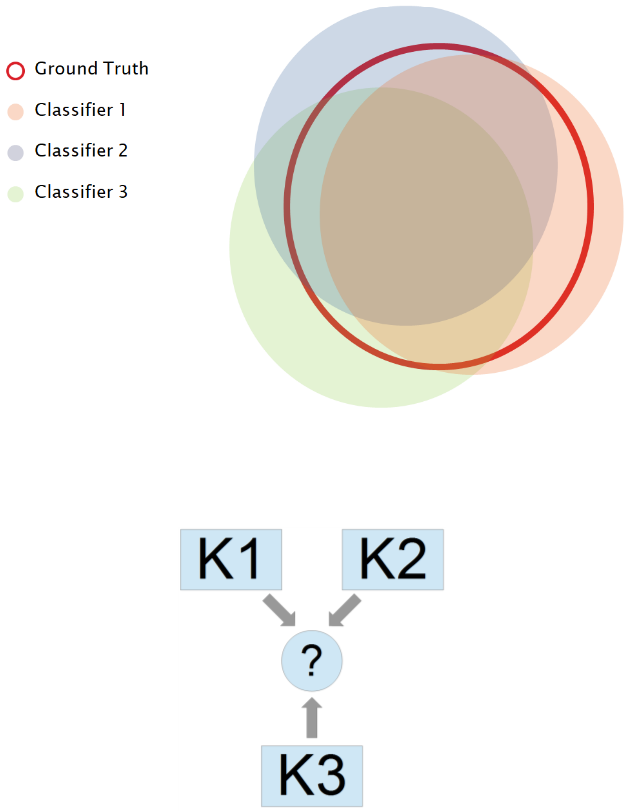
\includegraphics[height=5.2cm]{majorityvoting.png}
\end{figure}
\begin{block}
{}
\end{block}
\end{column}
\end{columns}

\end{frame}
















\section{Conclusion}

% nur für die Miniframe-Navigation
\subsection*{}

\begin{frame}
\frametitle{Comparison}
\begin{block}
{Accuracy of classification methods}
\end{block}
	\begin{table}

		\centering
			\begin{tabular}{cc}
				\toprule
				Classifier & Accuracy [\%] \\
				\midrule
				HMM & 66.7 \\
				SVM (full feature set) & 73.3 \\
				Majority Vote & 90.5 \\
				\bottomrule
			\end{tabular}
	\end{table}
	\begin{block}
	{}
	\end{block}
\end{frame}





\begin{frame}
\frametitle{Misclassifications}
\begin{figure}[!t]
\centering
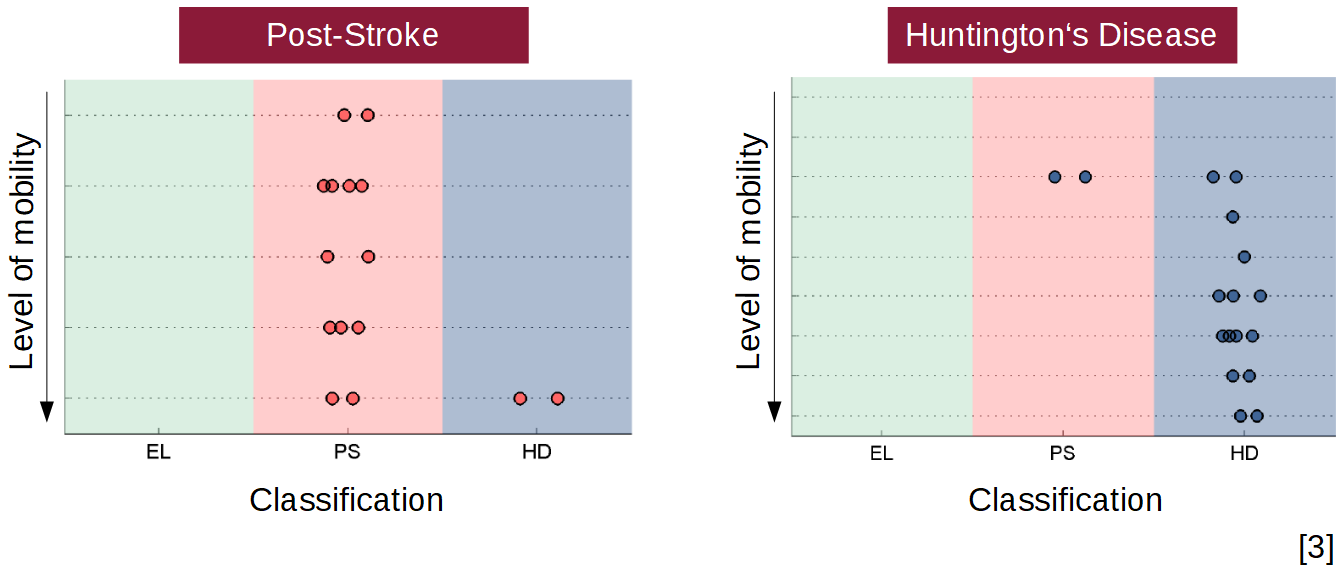
\includegraphics[height=4.2cm]{missclassification.png}
\end{figure}

\begin{block}
{$\Rightarrow$ for PS and HD, only between pathologic groups}
\end{block}
\end{frame}





\begin{frame}
\frametitle{Improvements}

\begin{block}
{$\blacktriangleright$ weighted votes based on classification uncertainty}
\end{block}

\begin{block}
{$\blacktriangleright$ further pathology groups to validate the framework}
\end{block}

\begin{block}
{$\blacktriangleright$ useage of spatial feature sets}
\end{block}

\end{frame}















% nur für die Miniframe-Navigation
\section*{}

\begin{frame}<beamer>{}
	\begin{center}
		Thanks for your attention!
	\end{center}
	\begin{center}
		Questions?
	\end{center}
\end{frame}











\begin{frame}
\frametitle {Sources}

{[1]	 - https://www.apdm.com/wearable-sensors/ (23.05.2018)  \newline http://kilograph.com/virtual-reality-6dof/ (23.05.2018)}



 {[2] - https://www.gettyimages.de/detail/video/male-body-walking-stock-videomaterial/618598925?esource=SEO\_GIS\_CDN\_Redirect (23.05.2018)}


{[3] - A Machine Learning Framework for Gait Classification Using Inertial Sensors: Application to Elderly, Post-Stroke and Huntington's Disease Patients: A. Mannini and D. Trojaniello and A. Cereatti and A. M. Sabatini, 21.01.2016 in Sensors 2016,16,134} 


\end{frame}


\end{document}